% Options Screener — Project Report
% Build:  tectonic docs/report/options_screener_report.tex
\documentclass[11pt,a4paper]{article}

% ---------------------------------------------------------------- packages
\usepackage{fontspec}
\setmainfont{texgyrepagella}[Extension=.otf,UprightFont=*-regular,BoldFont=*-bold,ItalicFont=*-italic,BoldItalicFont=*-bolditalic]
\setsansfont{texgyreheros}[Extension=.otf,UprightFont=*-regular,BoldFont=*-bold,ItalicFont=*-italic,BoldItalicFont=*-bolditalic]
\setmonofont{texgyrecursor}[Extension=.otf,UprightFont=*-regular,BoldFont=*-bold,ItalicFont=*-italic,BoldItalicFont=*-bolditalic,Scale=0.95]
\usepackage[a4paper,margin=2.3cm,headheight=14pt]{geometry}
\usepackage{xcolor}
\usepackage{tikz}
\usetikzlibrary{positioning,arrows.meta,shapes.geometric,calc,backgrounds,fit}
\usepackage{pgfplots}
\pgfplotsset{compat=1.18}
\usepackage[most]{tcolorbox}
\usepackage{booktabs,tabularx,array,multirow,colortbl}
\usepackage{enumitem}
\usepackage{fancyhdr}
\usepackage{titlesec}
\usepackage{microtype}
\usepackage[hidelinks]{hyperref}
\usepackage{eso-pic}

% ---------------------------------------------------------------- palette
\definecolor{ink}{HTML}{1B2430}
\definecolor{navy}{HTML}{14325C}
\definecolor{teal}{HTML}{1F7A8C}
\definecolor{gold}{HTML}{C9A227}
\definecolor{good}{HTML}{2E7D4F}
\definecolor{bad}{HTML}{B23A3A}
\definecolor{warn}{HTML}{C77D1A}
\definecolor{mist}{HTML}{EEF2F6}
\definecolor{rule}{HTML}{C5CED8}
\color{ink}

% ---------------------------------------------------------------- headings
\titleformat{\section}{\sffamily\Large\bfseries\color{navy}}
  {\colorbox{navy}{\color{white}\makebox[1.6em]{\thesection}}}{0.7em}{}
  [\vspace{-0.4em}{\color{rule}\rule{\textwidth}{0.6pt}}]
\titleformat{\subsection}{\sffamily\large\bfseries\color{teal}}{\thesubsection}{0.6em}{}
\titlespacing*{\section}{0pt}{1.6em}{0.9em}
\titlespacing*{\subsection}{0pt}{1.2em}{0.5em}

\pagestyle{fancy}
\fancyhf{}
\renewcommand{\headrulewidth}{0pt}
\fancyhead[L]{\sffamily\small\color{teal}Options Screener}
\fancyhead[R]{\sffamily\small\color{gray}Project report · 18 November 2026}
\fancyfoot[C]{\sffamily\small\color{gray}\thepage}

\setlist{itemsep=0.25em,topsep=0.4em,leftmargin=1.4em}
\setlength{\parskip}{0.45em}
\setlength{\parindent}{0pt}
\renewcommand{\arraystretch}{1.25}

% ---------------------------------------------------------------- boxes
\newtcolorbox{keybox}[1][]{enhanced,breakable,colback=mist,colframe=navy,
  boxrule=0pt,leftrule=3pt,arc=0pt,left=10pt,right=10pt,top=6pt,bottom=6pt,
  fonttitle=\sffamily\bfseries,coltitle=navy,colbacktitle=mist,
  attach title to upper={\par\smallskip},#1}
\newtcolorbox{alertbox}[1][]{enhanced,breakable,colback=bad!6,colframe=bad,
  boxrule=0pt,leftrule=3pt,arc=0pt,left=10pt,right=10pt,top=6pt,bottom=6pt,
  fonttitle=\sffamily\bfseries,coltitle=bad,attach title to upper={\par\smallskip},#1}
\newtcolorbox{goodbox}[1][]{enhanced,breakable,colback=good!6,colframe=good,
  boxrule=0pt,leftrule=3pt,arc=0pt,left=10pt,right=10pt,top=6pt,bottom=6pt,
  fonttitle=\sffamily\bfseries,coltitle=good,attach title to upper={\par\smallskip},#1}

\newcommand{\stat}[2]{%
  \begin{tcolorbox}[enhanced,colback=white,colframe=rule,boxrule=0.6pt,arc=2pt,
    width=\linewidth,halign=center,top=4pt,bottom=4pt]
    {\sffamily\bfseries\LARGE\color{navy}#1}\\[1pt]
    {\sffamily\footnotesize\color{gray}#2}
  \end{tcolorbox}}
\newcommand{\pill}[2]{\tikz[baseline=(t.base)]\node[fill=#1,text=white,rounded corners=1.5pt,
  inner sep=2pt,font=\sffamily\scriptsize\bfseries](t){#2};}
\newcommand{\CLOSED}{\pill{gray}{CLOSED}}
\newcommand{\PENDING}{\pill{warn}{PENDING}}
\newcommand{\LEAD}{\pill{teal}{LEAD}}
\newcommand{\BASE}{\pill{navy}{BASELINE}}
\newcommand{\FIXED}{\pill{good}{FIXED}}
\newcommand{\code}[1]{{\ttfamily\small #1}}

% ================================================================= document
\begin{document}

% ---------------------------------------------------------------- title page
\begin{titlepage}
\AddToShipoutPictureBG*{%
  \begin{tikzpicture}[remember picture,overlay]
    \fill[navy] (current page.north west) rectangle ([yshift=-11cm]current page.north east);
    % a stylised payoff diagram across the banner
    \begin{scope}[shift={([xshift=2.3cm,yshift=-10.5cm]current page.north west)},x=1cm,y=1cm]
      \draw[white!40!navy,line width=0.5pt] (0,1.2) -- (16.4,1.2);
      \draw[gold,line width=2pt,line cap=round] (0,0.2) -- (5.5,0.2) -- (8.2,2.4) -- (16.4,2.4);
      \draw[teal!70!white,line width=1.2pt,dashed] (0,2.0) .. controls (6,2.0) and (7,0.4) .. (16.4,0.4);
      \foreach \x in {0,1.2,...,16.4} \fill[white!30!navy] (\x,1.2) circle (0.9pt);
    \end{scope}
    \fill[gold] ([yshift=-11cm]current page.north west) rectangle ([yshift=-11.25cm]current page.north east);
  \end{tikzpicture}}
\vspace*{0.2cm}
{\color{white}\sffamily
  {\small\bfseries\color{gold} PROJECT REPORT · NOVEMBER 2026}\\[0.8em]
  {\fontsize{36}{40}\selectfont\bfseries Options Screener}\\[0.6em]
  {\Large A research system for finding, refusing and\\[0.2em] measuring options trades}
}
\vspace{8.4cm}

\begin{minipage}[t]{0.47\textwidth}
\sffamily\small
{\color{teal}\bfseries WHAT THIS DOCUMENT COVERS}\\[0.4em]
\begin{itemize}[leftmargin=1em]
  \item What the system is and how it is built
  \item The gates that decide what gets traded
  \item How the research is measured
  \item Every finding to date, with its status
  \item The state of the system on 18 Nov 2026
  \item What to do next, in priority order
\end{itemize}
\end{minipage}\hfill
\begin{minipage}[t]{0.47\textwidth}
\sffamily\small
{\color{teal}\bfseries THE ONE-LINE ANSWER}\\[0.4em]
After a year of work and about 1,000 paper trades, nothing has passed the
decision rule for real money. Every edge found so far is either real but
eaten by trading costs, or not real. What the system clearly does well is
\textbf{refuse expensive trades}.
\end{minipage}

\vfill
{\sffamily\footnotesize\color{gray}
Repository \code{Ollie1o1/options} · \code{main} at \code{e773314} (PR \#145)\\
compiled from \code{docs/report/options\_screener\_report.tex}}
\end{titlepage}

% ---------------------------------------------------------------- contents
\setcounter{tocdepth}{1}
\tableofcontents
\vspace{1em}

\begin{keybox}[title=Executive summary]
\textbf{What it is.} A Python system that scans US equity and ETF options chains,
scores candidate trades (single legs, vertical spreads, iron condors), passes
them through a series of refusal gates, and paper-trades the survivors on a
schedule. Every refused candidate is kept and followed to expiry as well, so the
gates themselves can be tested.

\textbf{Where it stands.} The paper book has closed 1,001 trades for
\textbf{+\$1,935}, profit factor 1.04 [0.87, 1.24]. That is not distinguishable from zero,
and it trails simply holding SPY. Real money is off by rule. Since 6 November the
book has made \textbf{no new entries}: Bull Puts are blocked, and every other candidate is
refused for negative expected value.

\textbf{What works.} The friction gate, which refuses trades whose bid-ask spread is
too large a share of the credit, is the largest effect measured anywhere in the
project (return on capital went from $-6.76\%$ to $-0.64\%$). The full gate also
reliably separates better credit spreads from worse ones on the same underlying and day.

\textbf{What needs attention now.} A scheduled job has been hung for 12 days, the
disk is 96\% full (it already ran out once, on 6 Nov), the health check reports the
auto-logger as OK when it is not, and gaps in the chain archive are costing the
March 2027 earnings test its data. Section~\ref{sec:next} has the list.
\end{keybox}

\newpage
% ================================================================= 1
\section{What the project is}

The screener began on 11 November 2025 as a tool to rank options by a weighted
blend of signals: volume, IV versus realised volatility, technical levels and
momentum, with an optional AI layer on top. Over the following year it changed
from a \emph{ranker} into a \emph{measuring instrument}. When the ranking was tested
out of sample, no ordering of the board beat a random draw ($p = 0.89$).
The project's guiding rule since then has been \textbf{refuse, don't rank}.
Candidates are filtered by gates that are known to help, survivors are sampled at
random, and every trade, whether taken or refused, is recorded so it can be judged later.

\begin{center}
\begin{minipage}{0.23\textwidth}\stat{102k}{lines of Python in \code{src/}}\end{minipage}\hfill
\begin{minipage}{0.23\textwidth}\stat{465}{test files}\end{minipage}\hfill
\begin{minipage}{0.23\textwidth}\stat{1,432}{commits · 145 PRs}\end{minipage}\hfill
\begin{minipage}{0.23\textwidth}\stat{13 GB}{of market data on disk}\end{minipage}
\end{center}

\subsection{Scope}
\begin{tabularx}{\textwidth}{@{}l X@{}}
\toprule
\textbf{Area} & \textbf{What it covers} \\
\midrule
Universe & 59 symbols in four watchlists (\emph{liquid large cap, sector ETFs, high IV, income}), widened to about 90 by discovery scans \\
Structures & Long Call, Long Put, Short Put, Bull Put, Bear Call, Iron Condor \\
Data & Yahoo/CBOE live chains; a daily chain archive; Dolt historical options; optionsDX SPY 2010--23; earnings and estimates archives; news and analyst actions \\
Ledgers & \code{paper\_trades.db} (the paper book) and \code{data/candidates.db} (3.4 GB shadow corpus of every candidate, taken or refused, with daily marks) \\
Automation & macOS launchd jobs for entry windows, exit enforcement, mark collection, chain archive, morning briefing and weekly checkpoint \\
Interfaces & Terminal "Quant Desk" launcher, HTML morning briefing and tear sheets, Discord/Telegram trade alerts \\
\bottomrule
\end{tabularx}

% ================================================================= 2
\section{How it is built}

\begin{center}
\begin{tikzpicture}[
  node distance=0.55cm and 0.5cm,
  box/.style={draw=navy,fill=white,rounded corners=2pt,line width=0.7pt,
     font=\sffamily\footnotesize,align=center,minimum height=1.0cm,text width=2.35cm},
  gate/.style={box,draw=bad,fill=bad!5,text width=2.2cm},
  store/.style={box,draw=teal,fill=teal!6,cylinder,shape border rotate=90,aspect=0.18,text width=2.2cm},
  arr/.style={-{Stealth[length=2.2mm]},line width=0.7pt,color=navy!80}]
  \node[box,fill=mist] (data) {\textbf{Market data}\\chains · prices\\earnings · news};
  \node[box,right=of data] (scan) {\textbf{Screener}\\score candidates\\EV after costs};
  \node[gate,right=of scan] (gates) {\textbf{Gates}\\friction · neg.\ EV\\earnings · sizing};
  \node[box,right=of gates] (alloc) {\textbf{Allocator}\\evidence weights\\random draw};
  \node[store,below=1.1cm of alloc] (book) {\textbf{Paper book}\\{\ttfamily\scriptsize paper\_trades.db}};
  \node[store,below=1.1cm of gates] (shadow) {\textbf{Shadow corpus}\\{\ttfamily\scriptsize candidates.db}};
  \node[box,below=1.1cm of scan,fill=mist] (marks) {\textbf{Daily marks}\\follow to expiry};
  \node[box,below=1.1cm of data,fill=gold!12,draw=gold!80!black] (research) {\textbf{Research}\\pre-registered\\tests};
  \draw[arr] (data) -- (scan);
  \draw[arr] (scan) -- (gates);
  \draw[arr] (gates) -- node[above,font=\sffamily\tiny]{passed} (alloc);
  \draw[arr] (alloc) -- (book);
  \draw[arr] (gates) -- node[right,font=\sffamily\tiny]{all, with reason} (shadow);
  \draw[arr] (marks) -- (shadow);
  \draw[arr] (shadow) -- ++(0,-1.1) -| (research);
  \draw[arr] (book) -- ++(0,-1.3) -| ([xshift=4mm]research.south);
  \draw[arr,dashed,gold!80!black] (research) -- node[left,font=\sffamily\tiny,align=right]{changes\\to gates} (data.south);
\end{tikzpicture}
\end{center}

The flow has five stages:
\begin{enumerate}
  \item \textbf{Scan.} \code{options\_screener.py} pulls chains, fits an IV surface
        (SVI), prices each candidate with Black--Scholes Greeks and a calibrated
        probability of profit, and computes expected value \emph{after} the bid-ask cost.
  \item \textbf{Gate.} \code{pick\_ranking.gate\_board} applies the refusal gates
        (next section). Each refusal is stored with its reason.
  \item \textbf{Allocate.} The allocator in \code{src/alloc/} weights strategies by their
        measured evidence (15\% exploration) and draws entries \emph{at random} among the
        survivors, so the logged trades stay an unbiased sample.
  \item \textbf{Size and log.} \code{book\_sizing.py} risks 2\% of equity per trade on
        capital at risk (never on premium), caps total open risk at 10\%, and refuses
        anything below one contract.
  \item \textbf{Measure.} Candidate marks follow every contract daily until expiry.
        Unmarked contracts settle at intrinsic value, and splits are voided.
        The research scripts in \code{scripts/} read both ledgers.
\end{enumerate}

\subsection{Module map}
{\small\begin{tabularx}{\textwidth}{@{}>{\raggedright\arraybackslash}X >{\raggedright\arraybackslash}p{4.6cm} l@{}}
\toprule
\textbf{Package} & \textbf{Role} & \textbf{Status} \\
\midrule
\code{options\_screener}, \code{scoring}, \code{spread\_scoring} & Scan, score and price candidates & live \\
\code{pick\_ranking}, \code{earnings\_gate}, \code{short\_premium\_gate} & Refusal gates & live \\
\code{alloc/}, \code{book\_sizing}, \code{strategy\_allocation} & Allocation by evidence; sizing & live \\
\code{candidate\_record}, \code{candidate\_marks}, \code{chain\_archive} & Shadow corpus and its marks & live \\
\code{maintenance}, \code{health}, \code{maintenance\_health} & Scheduling, alarms & live \\
\code{gate\_separation}, \code{benchmark/}, \code{policy\_lab/} & Research measurement & live \\
\code{morning/}, \code{tearsheet/}, \code{research/}, \code{trade\_alerts} & Briefings, reports, alerts & live \\
\code{crypto/}, \code{vol\_intel/}, \code{leverage/}, \code{breakout/}, \code{probability\_lab/} & Earlier lines of research & shelved \\
\bottomrule
\end{tabularx}}

% ================================================================= 3
\section{The gates}

The gates are where most of the measured value is. Each one refuses rather than
reorders. A refused candidate is still recorded and followed, so the gate can be
judged against what it turned away.

\begin{tabularx}{\textwidth}{@{}>{\bfseries}l X l@{}}
\toprule
Gate & What it refuses & Evidence \\
\midrule
Friction & Spreads where the round-trip bid-ask cost is more than 25\% of the credit & strongest effect in the project \\
Negative EV & Candidates whose expected value after costs is negative or marginal (\code{spread\_negative\_ev\_mode = refuse}) & separates at mid on its own \\
Earnings & Trades held through an announced report, including same-day after-close reports; covers long options since \#144 & E1-L: buying into earnings lost $-16\%$ \\
Sizing & Anything below one contract at 2\% risk; total open risk above 10\% & by construction \\
Top quintile (G6) & Score above the 0.742 cutoff & had never fired; fixed \#145 \\
Strategy block & Bull Put (since 15 Oct, ``costly beta'') & SPY 2010--23 \\
Cluster cap & Too much risk in one ticker or sector & \emph{report mode only} \\
\bottomrule
\end{tabularx}

\begin{goodbox}[title={The gate works, on a relative basis}]
Matched within the same underlying, expiry and day, a gate-passed credit spread beats a
refused one about 73\% of the time (Bear Call $+0.19$, Bull Put $+0.17$ on fresh
October--November data; family-wise $p<0.001$). The result held when the 11-10 audit removed
the weekend artefacts and repriced everything at mid. This is evidence that the gate picks
\emph{better} trades. It is not evidence that the trades it picks make money.
\end{goodbox}

% ================================================================= 4
\section{How the research is measured}

Most of the year's lessons came from finding measurements that were wrong. The
methods below exist because a simpler version produced a confident and wrong answer.

\begin{description}[style=nextline,leftmargin=1.2em,font=\sffamily\bfseries\color{teal}]
  \item[Pre-register, then look.] Each test has a written hypothesis, estimator and pass
        rule before its data is opened (\code{docs/PREREG\_*}). The decision rule of
        15 October requires a historical pass, then at least 8 forward weeks, then a
        \$1,500 pilot to measure real fills.
  \item[Capital at risk, never premium.] \code{pnl\_pct} is return on premium and is unbounded
        below for credit spreads (one Bull Put shows \code{pnl\_pct} = $-168.2$). All P\&L is judged on capital
        at risk.
  \item[Match, don't pool.] A pooled \code{GROUP BY gate\_passed} reverses sign through
        Simpson's paradox. Comparisons are matched within (symbol, expiry, day).
  \item[Beat your own delta.] A put spread is partly a long position in the underlying. Results
        are judged as \emph{excess} over holding the same delta in shares.
  \item[Cross the spread.] Paper fills at mid flatter every short-premium idea. The
        11-10 audit showed the headline Bear Call result was a mid-exit figure.
  \item[Count clusters, not rows.] Thousands of rows from one day are one observation of
        that day's market. Confidence intervals are clustered by day or month.
\end{description}

% ================================================================= 5
\section{What has been found}

\subsection{The paper book}

\begin{minipage}[c]{0.56\textwidth}
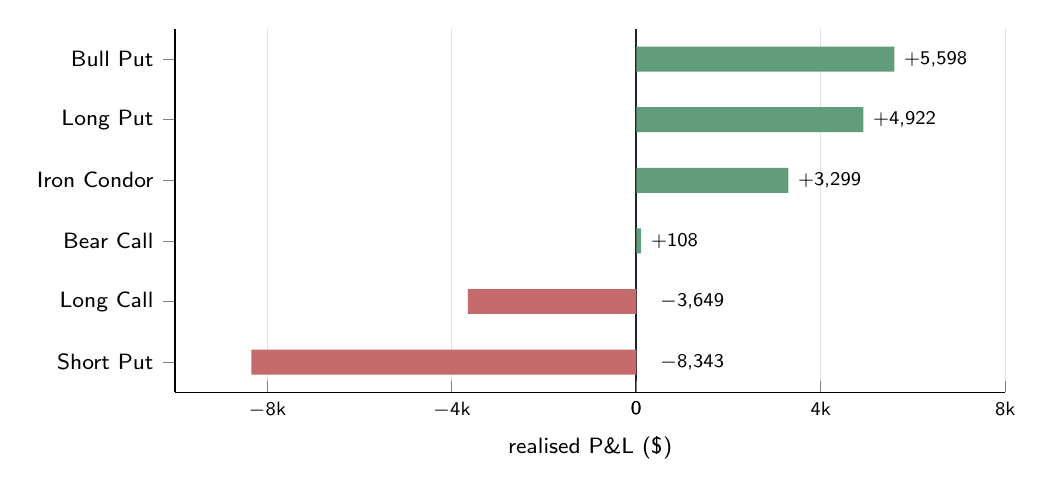
\begin{tikzpicture}
\begin{axis}[
  xbar, width=\linewidth, height=6.2cm,
  bar width=9pt, y dir=reverse,
  symbolic y coords={Bull Put,Long Put,Iron Condor,Bear Call,Long Call,Short Put},
  ytick={Bull Put,Long Put,Iron Condor,Bear Call,Long Call,Short Put}, bar shift=0pt,
  scaled x ticks=false, xtick={-8000,-4000,0,4000,8000},
  xticklabels={$-$8k,$-$4k,0,4k,8k}, yticklabel style={font=\sffamily\footnotesize},
  xticklabel style={font=\sffamily\scriptsize},
  xlabel={\sffamily\footnotesize realised P\&L (\$)},
  xmin=-10000, xmax=8000, axis x line*=bottom, axis y line*=left,
  xmajorgrids, grid style={rule!60},
  nodes near coords, nodes near coords style={font=\sffamily\scriptsize},
  every node near coord/.append style={anchor=west},
  point meta=explicit symbolic,
  extra x ticks={0}, extra x tick style={grid style={ink,line width=0.8pt}},
]
\addplot[fill=good!75,draw=none] coordinates {(5598,Bull Put)[+5,598] (4922,Long Put)[+4,922] (3299,Iron Condor)[+3,299] (108,Bear Call)[+108]};
\addplot[fill=bad!75,draw=none] coordinates {(-3649,Long Call)[] (-8343,Short Put)[]};
\node[font=\sffamily\scriptsize,anchor=west] at (axis cs:300,Long Call) {$-$3,649};
\node[font=\sffamily\scriptsize,anchor=west] at (axis cs:300,Short Put) {$-$8,343};
\end{axis}
\end{tikzpicture}
\end{minipage}\hfill
\begin{minipage}[c]{0.4\textwidth}
\sffamily\small
\textbf{1,001 closed trades}, 18 Apr -- 5 Nov 2026\\[0.3em]
Total realised: \textbf{+\$1,935}\\
Profit factor: \textbf{1.04} [0.87, 1.24]\\
vs.\ SPY over 5.4 months: \textbf{$-$\$7,700}\\[0.6em]
\normalfont\small
No strategy's result is significant once trades are equal-weighted. The headline
profit before sizing shipped came entirely from which trades happened to be large.
\end{minipage}

\subsection{Short-premium ideas, judged against their delta}

Each bar is excess return over holding the same delta, as a percentage of capital at risk per
trade, with its 95\% confidence interval. To pass, the whole interval has to sit to the right of zero.

\begin{center}
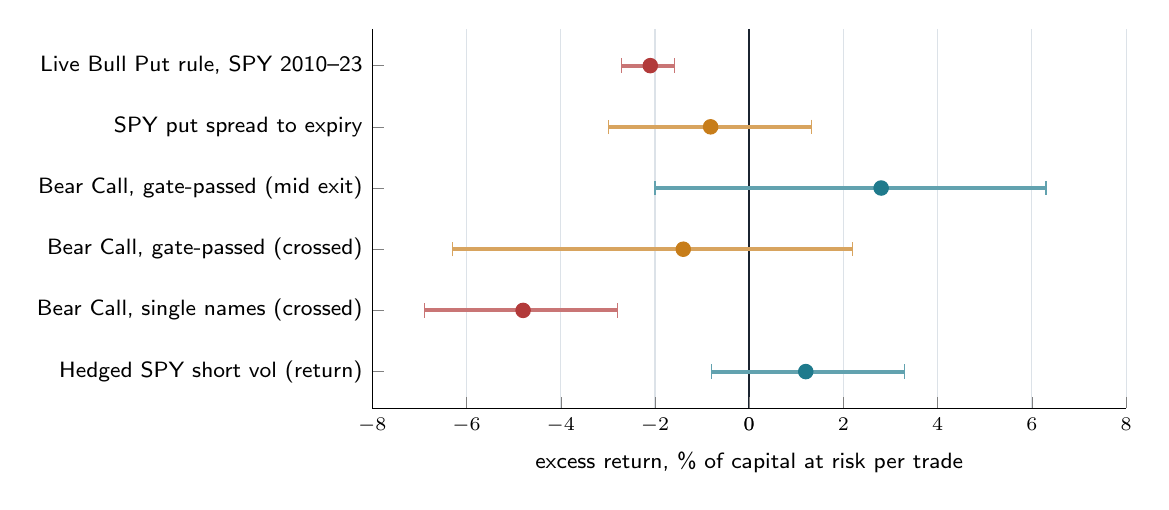
\begin{tikzpicture}
\begin{axis}[
  width=0.92\textwidth, height=6.4cm,
  y dir=reverse, ytick={1,...,6},
  yticklabels={
    {Live Bull Put rule, SPY 2010--23},
    {SPY put spread to expiry},
    {Bear Call, gate-passed (mid exit)},
    {Bear Call, gate-passed (crossed)},
    {Bear Call, single names (crossed)},
    {Hedged SPY short vol (return)}},
  yticklabel style={font=\sffamily\footnotesize,align=right},
  xticklabel style={font=\sffamily\scriptsize},
  xlabel={\sffamily\footnotesize excess return, \% of capital at risk per trade},
  xmin=-8, xmax=8, ymin=0.4, ymax=6.6,
  xmajorgrids, grid style={rule!60},
  axis y line*=left, axis x line*=bottom,
  extra x ticks={0}, extra x tick style={grid style={ink,line width=0.9pt}},
]
\addplot[only marks,mark=*,mark size=2.6pt,color=bad,
  error bars/.cd,x dir=both,x explicit,error bar style={line width=1.4pt,color=bad!70}]
  coordinates {(-2.10,1) -= (0.62,0) += (0.51,0)
               (-4.8,5) -= (2.1,0) += (2.0,0)};
\addplot[only marks,mark=*,mark size=2.6pt,color=warn,
  error bars/.cd,x dir=both,x explicit,error bar style={line width=1.4pt,color=warn!70}]
  coordinates {(-0.82,2) -= (2.16,0) += (2.14,0)
               (-1.4,4) -= (4.9,0) += (3.6,0)};
\addplot[only marks,mark=*,mark size=2.6pt,color=teal,
  error bars/.cd,x dir=both,x explicit,error bar style={line width=1.4pt,color=teal!70}]
  coordinates {(2.8,3) -= (4.8,0) += (3.5,0)
               (1.2,6) -= (2.0,0) += (2.1,0)};
\end{axis}
\end{tikzpicture}
\end{center}
{\small\color{gray} Red: reliably below zero. Amber: inconclusive, centred below zero. Teal: inconclusive, centred above
zero. The hedged-vol row is absolute return, not excess. At its effect size, confirming it would take about 39 years of data.}

\subsection{Directional signals, judged against the cost of trading}

\begin{center}
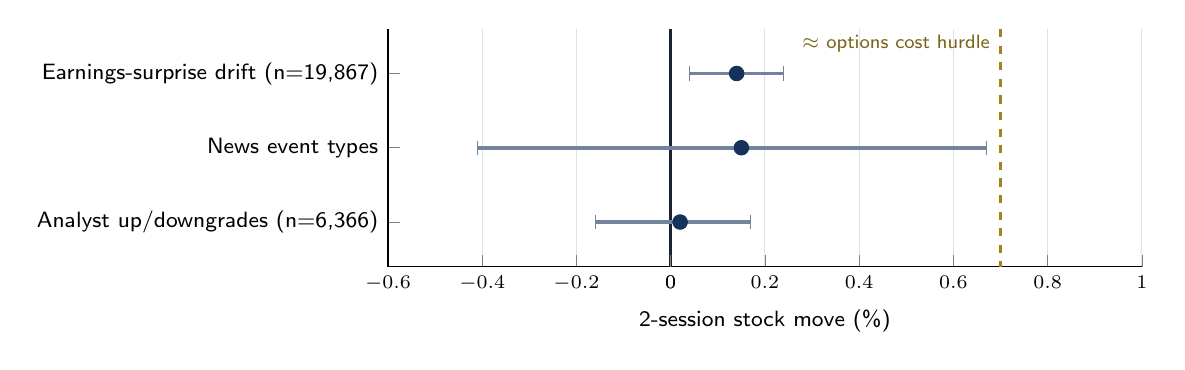
\begin{tikzpicture}
\begin{axis}[
  width=0.92\textwidth, height=4.6cm,
  y dir=reverse, ytick={1,2,3},
  yticklabels={{Earnings-surprise drift (n=19,867)},{News event types},{Analyst up/downgrades (n=6,366)}},
  yticklabel style={font=\sffamily\footnotesize},
  xticklabel style={font=\sffamily\scriptsize},
  xlabel={\sffamily\footnotesize 2-session stock move (\%)},
  xmin=-0.6, xmax=1.0, ymin=0.4, ymax=3.6,
  xmajorgrids, grid style={rule!60},
  axis y line*=left, axis x line*=bottom,
  extra x ticks={0}, extra x tick style={grid style={ink,line width=0.9pt}},
]
\addplot[only marks,mark=*,mark size=2.6pt,color=navy,
  error bars/.cd,x dir=both,x explicit,error bar style={line width=1.4pt,color=navy!60}]
  coordinates {(0.14,1) -= (0.10,0) += (0.10,0)
               (0.15,2) -= (0.56,0) += (0.52,0)
               (0.02,3) -= (0.18,0) += (0.15,0)};
\draw[gold!80!black,dashed,line width=1pt] (axis cs:0.70,0.4) -- (axis cs:0.70,3.6)
  node[pos=0.06,left,font=\sffamily\scriptsize,text=gold!60!black]{$\approx$ options cost hurdle};
\end{axis}
\end{tikzpicture}
\end{center}
Earnings drift is real but about five times too small to pay for an option's spread. The other two are null.
Predicting direction from public data is treated as exhausted here.

\subsection{Findings register}

\begin{tabularx}{\textwidth}{@{}l X l@{}}
\toprule
\textbf{Date} & \textbf{Finding} & \textbf{Status} \\
\midrule
Aug & Friction filter: return on capital $-6.76\% \to -0.64\%$ & \BASE \\
Aug & Single-name short vol: PF 0.30, no edge & \CLOSED \\
09-28 & Book trails SPY by \$7,700; PF 1.04 [0.87, 1.24] & \CLOSED \\
09-28 & 750 exit-rule combinations: none promoted; exits are second-order & \CLOSED \\
09-29 & Gate separates credit spreads (matched, $p<0.001$) & \CLOSED \\
09-30 & Bull Put scarcity is the EV gate, not the universe & \CLOSED \\
10-10..14 & Earnings drift, news, analyst actions, post-shock drift: null or below hurdle & \CLOSED \\
10-13 & Long options at 1--3 sessions lose about 8\% of premium, mostly the spread & \CLOSED \\
10-15 & Live Bull Put rule is costly beta ($-2.10\%$); auto-logging stopped & \CLOSED \\
10-15 & Decision rule: history $\to$ 8 forward weeks $\to$ \$1,500 pilot & \BASE \\
11-09 & Earnings premium: $+4\%$ at mid, $-20\%$ to $-33\%$ crossed & \CLOSED \\
11-09 & Earnings held to expiry is worse & \CLOSED \\
11-09 & Hedged SPY short vol: $+1.2\%$ [$-0.8$, $+3.3$], underpowered & \CLOSED \\
11-09 & Earnings filter was blind since 08-20; long options now gated & \FIXED \\
11-10 & Bear Call PF 1.89 is a mid-exit figure; crossed PF 1.19 [0.68, 2.24] & \LEAD \\
11-10 & Four shadow-corpus bugs (entry dates, stale-mark exits, G6, stale cache) & \FIXED \\
\bottomrule
\end{tabularx}

% ================================================================= 6
\newpage
\section{State of the system on 18 November 2026}

\begin{tabularx}{\textwidth}{@{}l l X@{}}
\toprule
\textbf{Check} & \textbf{Status} & \textbf{Detail} \\
\midrule
Code & \pill{good}{OK} & \code{main} = \code{e773314}; PR \#145 (11-10 audit) merged; no open PRs \\
Scheduled jobs & \pill{good}{OK} & Entry windows, checkpoint, track record, chain archive and briefing all ran today \\
Candidates & \pill{good}{OK} & 18,061 recorded in 7 days, 0 errors \\
Paper book & \pill{warn}{IDLE} & 0 open positions; last entry 5 Nov. Today's windows refused 68 of 71 spreads for negative EV, and Bull Puts are blocked \\
Candidate marks & \pill{bad}{CRITICAL} & 1,376 open positions never marked; 236 symbol/expiry pairs went dark on today's run \\
Chain archive & \pill{warn}{WARN} & 9 Nov lost for good; symbols per day down from 32 to about 21--26 \\
Allocation drift & \pill{warn}{WARN} & Long Put 33\% of the last 30 entries against a 16\% target \\
\bottomrule
\end{tabularx}

\begin{alertbox}[title=Found while writing this report]
\raggedright
\begin{enumerate}[leftmargin=1.2em]
  \item \textbf{A job has been hung for 12 days.} The launchd job
        \code{com.ollie.options.auto-log-equity} started \code{run.py -ss} on 6 Nov at 14:15 and never
        exited (PIDs 4771 and 4817). Its last log line is \code{OSError: [Errno 28] No space left on
        device}. launchd will not start a second copy while one is running, so this job has done nothing
        since. Its wrapper also still routes the 14:00--15:00 window to \code{-ss}, the Short Put window that \#136
        dropped from maintenance.
  \item \textbf{The disk is 96\% full,} with 8.4 GB free. The 6 Nov crash came from running out of space. \code{data/} holds
        13 GB: \code{optionsdx.db} 4.4 GB, \code{candidates.db} 3.4 GB (growing about 4,000 rows a day), \code{dolt\_options.db} 1.9 GB.
  \item \textbf{Two health checks disagree.} \code{maintenance -{}-health} reports auto-log as OK, last run today. The
        screener's start-up check says ``last ran 12 days ago''. Neither tells apart ``ran and refused everything''
        (correct, and what is happening) from ``did not run'' (the hung job).
\end{enumerate}
\end{alertbox}

% ================================================================= 7
\section{What could be done}\label{sec:next}

Ranked by value per hour. The first group is maintenance that protects the
measurements already scheduled. The second is research that could still change a
verdict. The last group is what \emph{not} to do, because each item has already been measured.

\subsection{Do now: protect the data}
\begin{enumerate}
  \item \textbf{Kill the hung job and retire or fix the launchd wrapper.} Kill with \code{kill 4817 4771}. Then either remove
        \code{com.ollie.options.auto-log-equity}, since maintenance already runs the entry windows, or wrap its
        \code{run.py} call in a time limit and drop the \code{-ss} branch.
  \item \textbf{Free disk space and alarm on it.} Move \code{optionsdx.db} and \code{optionsdx\_raw/}
        (4.8 GB, used only by closed research) to external storage. \code{VACUUM} \code{candidates.db}. Add a
        free-space line to \code{-{}-health} that warns below 15 GB.
  \item \textbf{Make the auto-log health check honest.} Stamp each window with \emph{ran / refused N / entered N}, and alarm when a
        launchd job's process is older than its interval.
  \item \textbf{Stop losing chain-archive days.} E2 (the March 2027 earnings test) has already lost 7 events. Add a
        second archive slot after the close, and either set the Mac to wake for it (\code{pmset repeat wakeorpoweron})
        or move the archiver to a machine that does not sleep.
  \item \textbf{Clear the 1,376 unmarked positions.} Check whether they are the same dark pairs (delisted or illiquid
        strikes) and let them settle at intrinsic, as \#134 does for expiries.
\end{enumerate}

\subsection{Next: research that could still change a verdict}
\begin{enumerate}[resume]
  \item \textbf{Register the estimate-revisions test before mid-January.} The archive has been collecting since 14 Oct,
        but there is no written hypothesis and no estimator. Write the hypothesis before opening the data.
  \item \textbf{Decide the B1-F rule now.} Does a Bear Call forward pass on 20 Jan also have to hold at crossed fills? The audit
        says it should, because every other test was judged crossed. Settling this before the data arrives keeps the test honest.
  \item \textbf{Work on execution cost, the one lever left.} Every edge found dies at the bid-ask. Measure what a patient
        limit order actually fills at: log limit orders at 25\% and 50\% of the half-spread on liquid ETFs and record
        how many fill. If index Bear Calls fill near mid, the 1.41 ETF profit factor becomes a real question.
  \item \textbf{More index history.} The hedged SPY short-vol test was underpowered (needs about 39 years of data). Adding SPX
        from 2004 and other index underlyings (QQQ, IWM) is the cheapest way to add power.
  \item \textbf{Use the own-picks scorecard.} \code{own\_picks.db} is still empty. Logging even 20 manual swing picks would show
        whether discretion beats the board at the 1--3 session horizon you actually trade.
\end{enumerate}

\subsection{Don't: already measured}
\begin{itemize}
  \item Widen the Bull Put universe, re-tune the friction ceiling, or sweep exits again
  \item Hunt for new single features, or re-run the direction signals on the same window
  \item Rank the board. Refuse-don't-rank stands ($p = 0.89$)
  \item Flip \code{cluster\_cap\_mode} to refuse (it has not fired), or turn on real money before the decision rule is passed
\end{itemize}

% ================================================================= 8
\newpage
\section{Upcoming checks}

\begin{center}
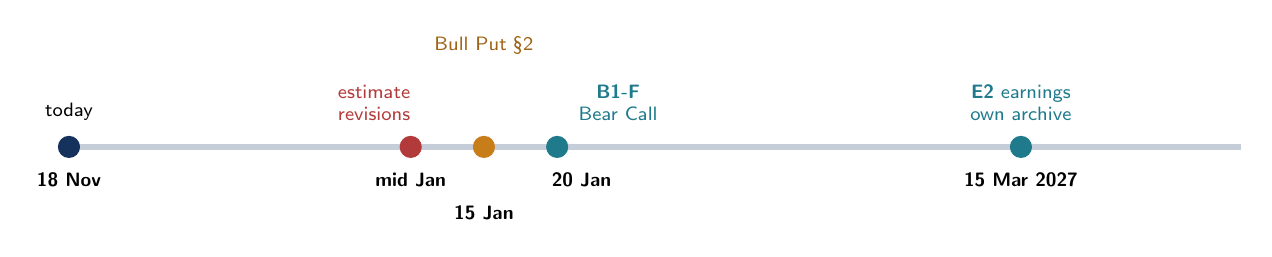
\begin{tikzpicture}[x=1.55cm]
  \draw[line width=2pt,color=rule] (0,0) -- (9.6,0);
  \foreach \x/\d/\t/\c in {
      0/{18 Nov}/{today}/navy,
      2.8/{mid Jan}/{estimate revisions\\(register first)}/bad,
      3.4/{15 Jan}/{Bull Put §2\\new empty cache}/warn,
      4.0/{20 Jan}/{\textbf{B1-F Bear Call}\\forward}/teal,
      7.8/{15 Mar}/{\textbf{E2 earnings}\\own archive}/teal} {
    \fill[\c] (\x,0) circle (4pt);
  }
  \node[font=\sffamily\scriptsize\bfseries,below=6pt] at (0,0) {18 Nov};
  \node[font=\sffamily\scriptsize,above=6pt,align=center] at (0,0) {today};
  \node[font=\sffamily\scriptsize\bfseries,below=6pt] at (2.8,0) {mid Jan};
  \node[font=\sffamily\scriptsize,above=6pt,align=center,text=bad] at (2.5,0) {estimate\\revisions};
  \node[font=\sffamily\scriptsize\bfseries,below=18pt] at (3.4,0) {15 Jan};
  \node[font=\sffamily\scriptsize,above=30pt,align=center,text=warn!80!black] at (3.4,0) {Bull Put §2};
  \node[font=\sffamily\scriptsize\bfseries,below=6pt] at (4.2,0) {20 Jan};
  \node[font=\sffamily\scriptsize,above=6pt,align=center,text=teal] at (4.5,0) {\textbf{B1-F}\\Bear Call};
  \node[font=\sffamily\scriptsize\bfseries,below=6pt] at (7.8,0) {15 Mar 2027};
  \node[font=\sffamily\scriptsize,above=6pt,align=center,text=teal] at (7.8,0) {\textbf{E2} earnings\\own archive};
\end{tikzpicture}
\end{center}

\begin{tabularx}{\textwidth}{@{}l >{\raggedright\arraybackslash}X@{}}
\toprule
\textbf{When} & \textbf{Command} \\
\midrule
$\ge$ 15 Jan & \code{python -m scripts.delta\_matched\_benchmark -{}-cache NEW\_EMPTY\_DIR -{}-exit-through 2027-01-15} \\
mid Jan & Estimate revisions: \emph{write the registration first; no estimator exists yet} \\
$\ge$ 20 Jan & \code{python -m scripts.bear\_call\_absolute -{}-cache DIR -{}-forward} (prints the crossed-fill line) \\
$\ge$ 15 Mar & \code{python -m scripts.earnings\_premium\_dolt -{}-forward} (\code{-{}-coverage} any time) \\
\bottomrule
\end{tabularx}

% ================================================================= A
\appendix
\section{Running it}

All commands run from \code{\textasciitilde/Projects/options} with the venv at \code{\textasciitilde/.venvs/options/bin/python} and
\code{PYTHONPATH=\$PWD}.

\begin{tabularx}{\textwidth}{@{}>{\raggedright\arraybackslash}p{7.2cm} >{\raggedright\arraybackslash}X@{}}
\toprule
\code{-m src.options\_screener} & Interactive screener (non-interactive: \code{-{}-mode discover -{}-weights baseline -{}-auto -{}-no-ai}) \\
\code{-m src.maintenance -{}-health} & Job, marks, archive and allocation health \\
\code{-m src.check\_pnl} & Paper book P\&L \\
\code{-m src.own\_picks -{}-log T DATE K call|put -{}-price P} & Log a manual pick \\
\code{-m scripts.gate\_separation\_report} & Matched gate-separation test \\
\code{scripts/run\_tests.py <substring>} & Test a group of the suite (the single-process run hangs on this Mac) \\
\bottomrule
\end{tabularx}

\begin{keybox}[title=Caution]
\code{run.py -ds}, \code{-sps} and \code{-ss} include \code{-{}-auto-log -{}-log-top 5} and enter paper trades. A bare
\code{python -m unittest tests.test\_maintenance} writes to the real \code{candidates.db}. Use \code{scripts/run\_tests.py}.
\end{keybox}

\end{document}
